%HI BENNI, this first part will be moved later, but I put it here to avoid merge problems
\begin{frame}{Test Cases}
\begin{figure}
%\vspace{-.7cm}	
%\hspace{-2cm}
		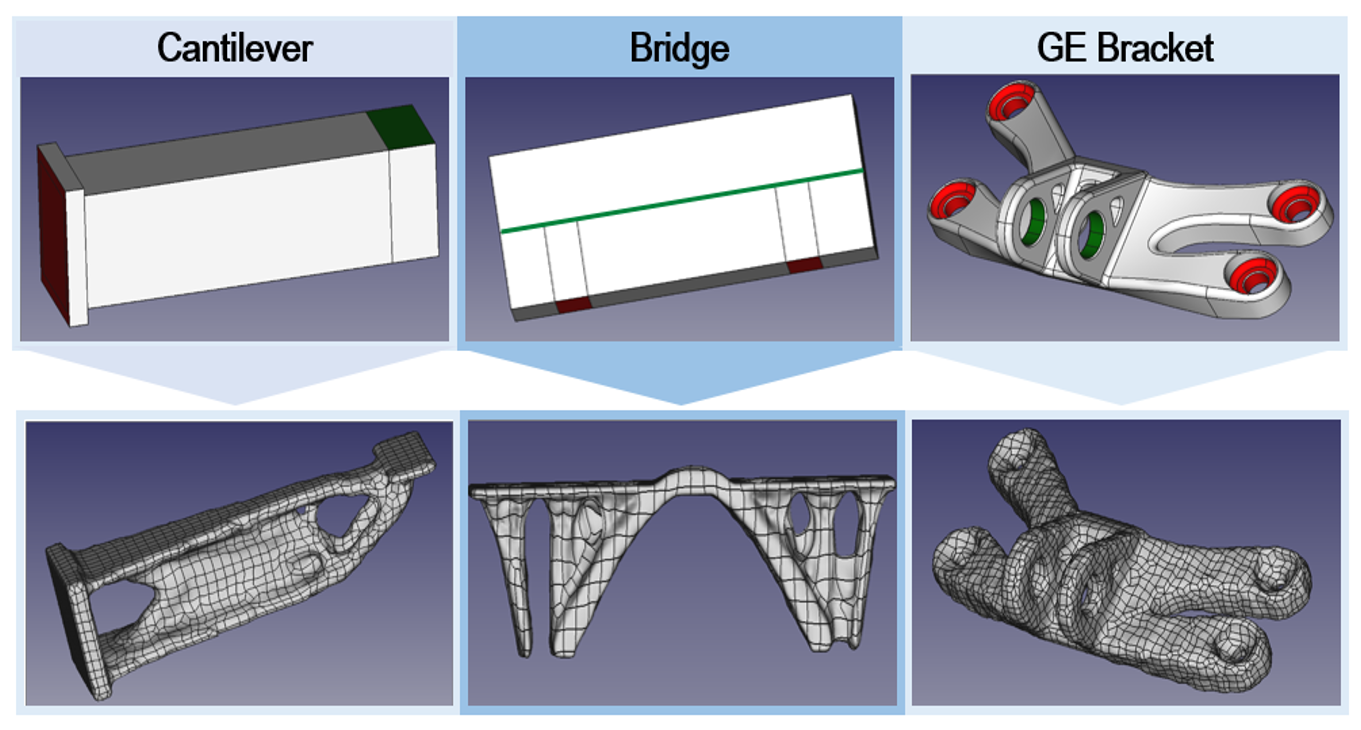
\includegraphics[width=1\linewidth]{Pictures/SecondHalf/TestCases.png}
		\end{figure}

\end{frame}
\begin{frame}
\begin{figure}

\vspace{-.7cm}	
\hspace{-2cm}		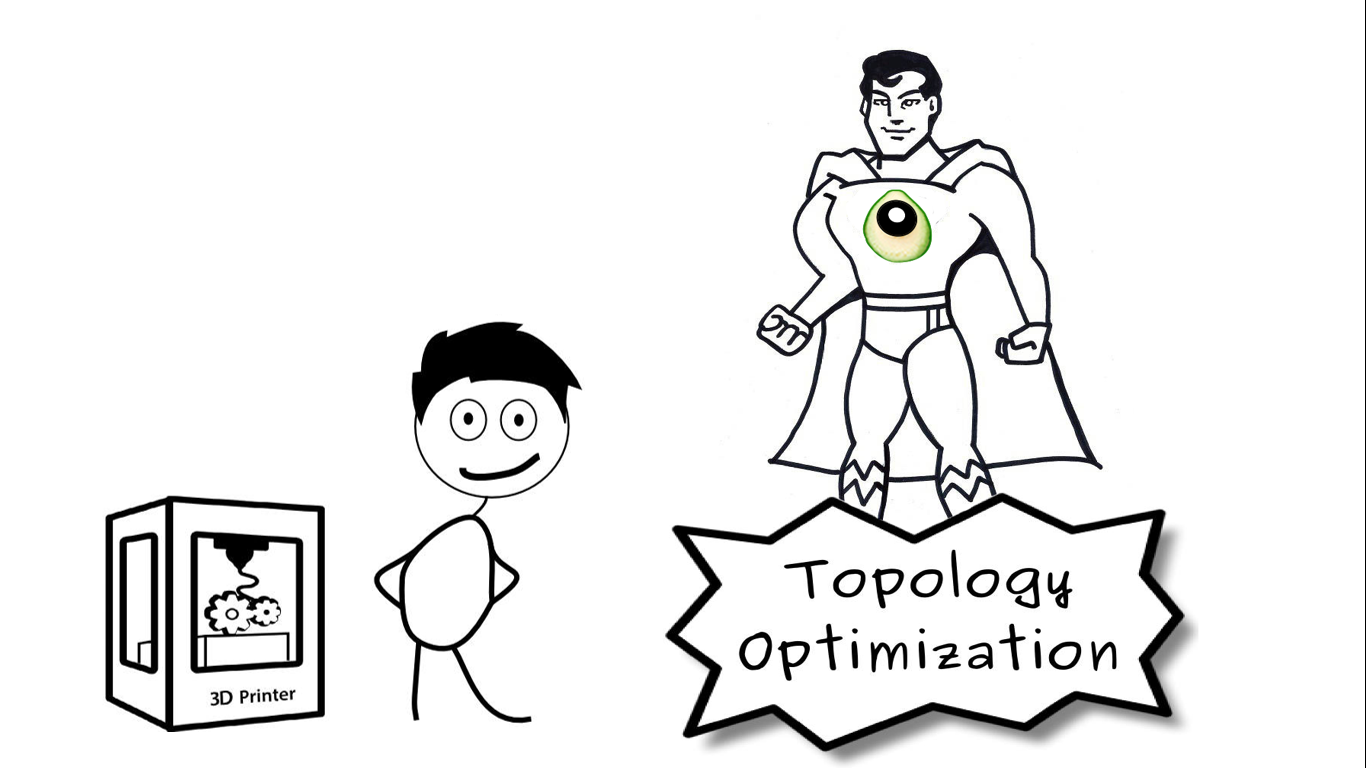
\includegraphics[width=1.2\linewidth]{Pictures/animations/animation_10.png}
		\end{figure}

\end{frame}

\begin{frame}{Third Milestone's achievements}
%\begin{variableblock}{What's done?}{bg=cyan,fg=white}{bg=white,fg=black}
%{



\begin{itemize}
	\item[\textcolor{green}{\Checkmark}] Fully integrated pipeline 
	
	\item[\textcolor{green}
	{\Checkmark}] Boolean operation support
		
	\item[\textcolor{green}
	{\Checkmark}] GUI for user interaction
	
	\item[\textcolor{green}
	{\Checkmark}] Fairness functional to control Peters' scheme smoothness
	
		\item[\textcolor{green}
	{\Checkmark}] Conversion back to CAD
	
	\item[\textcolor{green}
	{\Checkmark}] Test Cases


\end{itemize}

\end{frame}

\begin{frame}{Outlook \& future work}
\begin{itemize}
\item Make surface reconstruction more robust
\item Improve parameter estimation
\begin{itemize}
\item[--] complexity of algorithm 
\item[--] accuracy of result
\end{itemize}
\item Determine approximation error for our algorithm
\begin{itemize}
\item[--] Topology checks
\item[--] Accuracy estimates
\end{itemize}
\item Develop a fully adaptive scheme
\item Exchange ToPy with a faster solution
\end{itemize}
\end{frame}





%%%%%%%%%%%%%%%%%%%%%%%%%%%%%%%%%%%%%%%
%%%OLD SLIDES

%\begin{frame}{What is next?}
%\begin{variableblock}{What's done?}{bg=cyan,fg=white}{bg=white,fg=black}
%{
%\begin{itemize}

%\item<+-> Topology Optimization
%\begin{itemize}
%	\item[\textcolor{green}{\Checkmark}] Pipeline from CAD model to optimized voxel model
%	\item[\textcolor{green}{\Checkmark}] User input of boundary conditions
%	\item[\textcolor{black}{\VarClock}] Support for complex geometries
%	\item[\textcolor{red}{\XSolidBrush}] GUI for user interaction
%\end{itemize}

%\item<+-> Surface Extraction
%\begin{itemize}
%	\item[\textcolor{green}{\Checkmark}] Dual Contouring for simple geometries
%	\item[\textcolor{green}{\Checkmark}] Provide necessary data for Surface Fitting
%	\item[\textcolor{black}{\VarClock}] Interfaces
	%\item[\textcolor{red}{\XSolidBrush}] Adaptive and topology safe Dual Contouring
%\end{itemize}

%\item<+-> Surface Fitting
%\begin{itemize}
	%\item[\textcolor{green}{\Checkmark}] B--spline fitting using least squares
	%\item[\textcolor{green}{\Checkmark}] Smooth connection of patches using Peters' scheme
	%\item[\textcolor{red}{\XSolidBrush}] Conversion back to CAD
%\end{itemize}
%\end{itemize}
%}
%\end{variableblock}
%\end{frame}
















